\begin{pastexam}[label={px:ncku-108-ee-ds-09}]{成大電機所 108 學年度 問答題第 8 題}
（問答）

Please compute the shortest distances from A to all the other nodes in the following graph. Please
show your answer step by step. (15 points)

\begin{center}
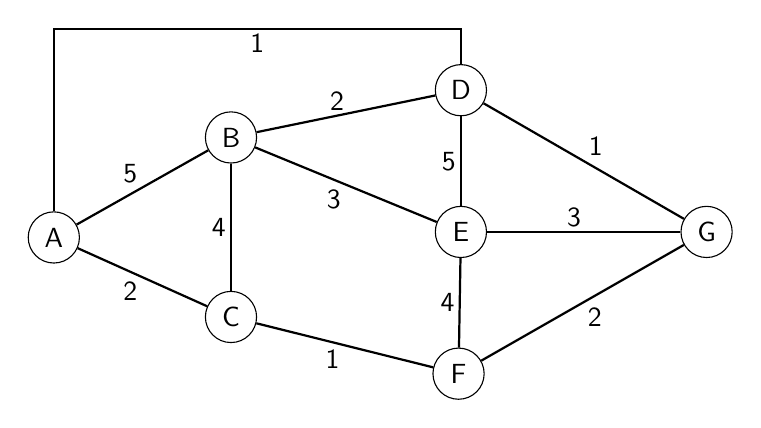
\begin{tikzpicture}[v/.style={circle,draw,minimum size=6.5mm,inner sep=0pt,font=\sffamily},w/.style={font=\sffamily,inner sep=1.5pt}]
\node[v] (A) at (5.18,-6.07) {A};
\node[v] (B) at (7.43,-4.80) {B};
\node[v] (C) at (7.43,-7.08) {C};
\node[v] (D) at (10.35,-4.20) {D};
\node[v] (E) at (10.35,-6.00) {E};
\node[v] (F) at (10.32,-7.80) {F};
\node[v] (G) at (13.47,-6.00) {G};
\draw[thick] (A) to node[w,above left] {5} (B);
\draw[thick] (A) to node[w,below left] {2} (C);
\draw[thick] (B) to node[w,above,pos=0.45] {2} (D);
\draw[thick] (B) to node[w,left] {4} (C);
\draw[thick] (B) to node[w,below left] {3} (E);
\draw[thick] (D) to node[w,left] {5} (E);
\draw[thick] (D) to node[w,above right] {1} (G);
\draw[thick] (E) to node[w,above,pos=0.45] {3} (G);
\draw[thick] (E) to node[w,left] {4} (F);
\draw[thick] (C) to node[w,below left] {1} (F);
\draw[thick] (F) to node[w,below right] {2} (G);
\draw[thick] (A) -- (5.18,-3.42) -- node[w,below] {1} (10.35,-3.42) -- (D);
\end{tikzpicture}
\end{center}
\end{pastexam}

\begin{pastsoln}
圖是無向圖，權重都是正的，用 Dijkstra 演算法（資結書第~25.2~節、虛擬碼~25.3）。 邊：$AB\,5$、$AC\,2$、$AD\,1$
（上方繞過去的那條）、$BC\,4$、$BD\,2$、$BE\,3$、$CF\,1$、$DE\,5$、$DG\,1$、$EF\,4$、$EG\,3$、$FG\,2$。

每一步從還沒確定的頂點裡取出 $d$ 最小的 $u$，確定它的距離，再用 $u$ 的邊鬆弛鄰居：$d[v] > d[u] + w(u,v)$
就更新 $d[v]$ 和前一個頂點 $\pi[v]$。 下表每一列是取出 $u$ 並鬆弛之後的 $d$，括號裡是 $\pi$；粗體表示這一步
確定的距離，「--」表示之前已確定。 距離相同時取字母小的（不影響最後的距離）。

\begin{center}
\small
\begin{tabular}{cc*{7}{c}}
\toprule
步 & 取出 & A & B & C & D & E & F & G \\
\midrule
0 & & 0 & $\infty$ & $\infty$ & $\infty$ & $\infty$ & $\infty$ & $\infty$ \\
1 & A & \textbf{0} & 5 (A) & 2 (A) & 1 (A) & $\infty$ & $\infty$ & $\infty$ \\
2 & D & -- & 3 (D) & 2 (A) & \textbf{1} & 6 (D) & $\infty$ & 2 (D) \\
3 & C & -- & 3 (D) & \textbf{2} & -- & 6 (D) & 3 (C) & 2 (D) \\
4 & G & -- & 3 (D) & -- & -- & 5 (G) & 3 (C) & \textbf{2} \\
5 & B & -- & \textbf{3} & -- & -- & 5 (G) & 3 (C) & -- \\
6 & F & -- & -- & -- & -- & 5 (G) & \textbf{3} & -- \\
7 & E & -- & -- & -- & -- & \textbf{5} & -- & -- \\
\bottomrule
\end{tabular}
\end{center}

每一步的鬆弛：
\begin{enumerate}
\item 取出 A（$0$）：$d[B] = 5$、$d[C] = 2$、$d[D] = 1$。
\item 取出 D（$1$）：B：$1 + 2 = 3 < 5$，更新；E：$1 + 5 = 6$；G：$1 + 1 = 2$。
\item 取出 C（$2$，和 G 同為 $2$，取 C）：B：$2 + 4 = 6$，不比 $3$ 小；F：$2 + 1 = 3$。
\item 取出 G（$2$）：E：$2 + 3 = 5 < 6$，更新；F：$2 + 2 = 4$，不比 $3$ 小。
\item 取出 B（$3$，和 F 同為 $3$，取 B）：E：$3 + 3 = 6$，不比 $5$ 小。
\item 取出 F（$3$）：E：$3 + 4 = 7$，不比 $5$ 小。
\item 取出 E（$5$），沒有未確定的鄰居，結束。
\end{enumerate}

\textbf{結果}（由 $\pi$ 倒推出最短路徑）：
\begin{center}
\begin{tabular}{ccl}
\toprule
頂點 & 距離 & 最短路徑 \\
\midrule
B & 3 & A $\to$ D $\to$ B \\
C & 2 & A $\to$ C \\
D & 1 & A $\to$ D \\
E & 5 & A $\to$ D $\to$ G $\to$ E \\
F & 3 & A $\to$ C $\to$ F \\
G & 2 & A $\to$ D $\to$ G \\
\bottomrule
\end{tabular}
\end{center}
到 E 的其他路徑，例如 A $\to$ D $\to$ E（$6$）、A $\to$ D $\to$ B $\to$ E（$6$）、A $\to$ C $\to$ F $\to$ E（$7$），都比 $5$ 長。
\end{pastsoln}
